
\section{复习}
\chat{%
国庆少了一节课。前面三次课回顾了历史、量子力学的公设、简单的一维体系。
}
\courseTime{Oct. 10, 2022\\Week 6\\4th}

量子力学公设,

1. 微观体系均可用含时的品优波函数描述,品优指单值连续有限,品优也是很多解的物理源头。

2. 任何可观测的力学量都对应线性算符,等于平均值。
\begin{eqnarray}
    \langle\hat{F}\rangle=\int_{-\infty}^{+\infty} \varphi^* \hat{F} \varphi d \tau=\langle\varphi|\hat{F}| \varphi\rangle
\end{eqnarray}

3. 一个算符作用到任何一个状态波函数,等于常数乘波函数,称这个波函数是本征函数。任何任意一个线性的厄米算符,那本征方程是
\begin{equation}
    \hat F \psi_i = \lambda_i \psi_i,
\end{equation}
并且它的本征函数构成完备集 $\{\psi_i\}$

4. 如果这个本征方程是厄米算符的本征方程,那么它有正交归一的性质,
\begin{align}
    \langle\psi_i | \psi_j \rangle = \delta_{ij} = \begin{cases}
        1, \quad &i = j, \\
        0, \quad &i\neq j,
    \end{cases}
\end{align}

% 4. 厄米算符有正交归一的性质
% \begin{eqnarray}
%     \hat F \psi_i = \lambda_i \psi_i, 
% \end{eqnarray}

\chat{%
从这个量子力学公设出发,我们可以知道量子化学里最重要的一个定态方程——薛定谔定态方程 $\hat H \psi_i = E_i \psi_i$。它是哈密顿算符的本征函数,哈密顿算符包含了动能项跟势能项,
\begin{eqnarray}
    \hat H = \hat T + \hat V = - \frac{\hbar^2}{2m}\pdv[2]{x} + \hat V
\end{eqnarray}
其中,对于单电子体系,动能算符是系统无依赖的算符。
但是体系的不同完全是由势能算符来给定的,所以不同的势能就对应的不同的体系。

在上一周课,我们讲了一维的量子体系。如果我们想要了解一个微观体系的信息,我们首先必须给出这个量子体系的薛定谔方程,这就是量子力学体系的状态波函数。对于量子力学的状态波函数的求解,需要通过定态许欸那个方程。而定态薛定谔方程的构建,最重要的一点就是对于势函数的构建。所以不同的量子力学体系,本质上就对应于不同的势函数以及势函数所对应的边界条件。}

最简单的一维量子力学体系,就是所谓的无限深势阱,如图 \ref{fig:inf_well}。
% 上周讲了一维的量子体系,
% 【】
% 必须给出状态波函数。通过定态薛定谔方程构建,关键就是势能函数、边界条件。最简单的一维量子体系是一维无线深势阱,【图】
\begin{align}
    V(x) = 
    \begin{cases}
        0, \quad &x\in[0,l],\\
        +\infty, \quad &\text{other}
    \end{cases}
\end{align}
能量 \begin{align}
    E_i = \frac{\hbar^2\pi^2 i^2} {2ml^2}, i = 1,2,3,\cdots,
\end{align}能得到零点能。

上周还讲了单侧无限深势阱,其一侧是无穷大,另一侧是有限的 $V_0$,如图 \ref{fig:half_inf_well}。这个体系的波函数比无限深势阱更复杂一些,势能表达式为
\begin{align}
    V(x) = 
    \begin{cases}
        \infty, \quad & x \in (-\infty, 0),\\
        0, \quad&x \in [0,l],\\
        V_0, \quad &\text{其它},
    \end{cases}
\end{align}
其能量满足的是
\begin{align}
    \cot z = -\sqrt{\left( \frac{z_0}z \right)^2 - 1}
\end{align}
超越方程,其中
\begin{align}
    z = \frac l\hbar \sqrt{2 m E}, \quad z_0 = \frac{l}{\hbar} \sqrt{2mV_0},
\end{align}
通过求解这个超越方程,能给出能量的量子化。$\{z_i\}$ 是量子化的,可求出能量 $E_i = \frac{\hbar^2 z_i^2}{2ml^2}$。

这个超越方程的形状、求解,上周有讲过。它的右边,当 $z \rightarrow0$ 时是无穷大,并且截止到 $z_0$,左边是 $\cot$ 函数,周期为 $\pi$,左右两边函数的交点就是解。当 $z_0 < \frac{\pi}2$ 时,没有交点,没有解,此时无法束缚。我们知道 $z_0$ 与 $V_0$ 有关,也就是当 $V_0$ 足够小的时候,是不能束缚住粒子的。当 $z_0 = \frac{\pi}2$ 时,系统可以束缚住粒子,此时解为 $z_1 = \frac{\pi}2$。当 $z_0 \geqslant \frac{\pi}2$ 时才有解,
\begin{align}
    z_0 = \frac{l}{\hbar} &\geqslant \frac{\pi}2 \\
    \frac{l^2}{\hbar^2} 2 m V_0 &\geqslant \frac{pi^2}4 \\
    V_0 &\geqslant \frac14 \frac{\hbar^2\pi^2}{2ml^2},
\end{align}
最小的束缚态能量为零点能的 1/4,即
\begin{align}
    V_0^{\text{min}} = \frac14 E_1,
\end{align}

\begin{figure}[tp]\centering
    \begin{tikzpicture}[scale=1.0]
        % axis
        \draw[->] (-0.2,0) -- (3.1, 0);
        \draw[->] (0,-0.2) -- (0, 2);
        \node[below] at (3.1,0) {$r$};
        % \fill[lightgray] (-2,0) rectangle (0,3);
        % \fill[lightgray] (0,0) rectangle (3,2);
        % % potential
    
        \draw[thick,fudanBlue] (0.5,0) -- (0.5,2);
        \draw[thick,fudanBlue] (0.5,0) -- (1.5,0);
        \draw[thick,fudanBlue] (1.5,0) -- (1.5,1);
        \draw[thick,fudanBlue] (1.5,1) -- (3.0,1);
        
        % \node[below] at (3,0) {$l$};
        % functions
        \draw[domain=0.45:3,thick,samples=100] plot (\x,{(1 - exp(-1.5* (\x - 1)))^2});
        \node[below] at (1.0,0) {$r_{\mathrm e}$};
        \node[right,fudanBlue] at (3.0,1) {$D_{\mathrm e}$};
    
    \end{tikzpicture}
    \caption{分子间势能与半无限深势垒}
\end{figure}
这个半无限深的模型体系有什么用呢?可以类比化学键的行为。以氢气为例,
\begin{align}
    \text{键能} \quad &D_{\mathrm e} = \SI{4.74}{\electronvolt}\\
    \text{零点能} \quad &\SI{0.26}{\electronvolt}\\
    \text{平衡位置} \quad &r_{\mathrm e} = \SI{0.7414}{\angstrom}
\end{align}把氢气用这个半无限深势阱描述,其中单位换算为
\begin{align}
    & m = \SI{1.673E-27}{\kilo\gram}, \quad \mu = \frac{m}2, \\
    & \hbar = \SI{1.055E-34}{\joule\second},\\
    & \SI{1}{\electronvolt} = \SI{1.602E-19}{\joule},
\end{align}
这里的 $\mu$ 是氢分子的折合质量,满足
\begin{align}
    \frac1\mu = \frac1{m_{\mathrm H}} + \frac1{m_{\mathrm H}}, 
\end{align}
代入数据,得到
\begin{align}
    z_0 &= \frac{l}{\hbar} \sqrt{2 m V_0} \notag\\
    &= \frac{\SI{0.5E-10}{\metre}}{\SI{1.055E-34}{\joule\second}} \sqrt{
        \SI{1.673E-27}{\kilo\gram} \times 
        \SI{4.74}{\electronvolt} \times
        \SI{1.602E-19}{\joule\per\electronvolt}
    } \notag\\
    &\approx 23.89 \approx 7.6 \pi,
\end{align}
当 $z_0$ 很大时,$z_1$ 接近于 $\pi$,也就是接近于无限深势阱的 $z_1$。

应用量子化条件,得到零点能
\begin{equation}
    E_1 = \frac{\hbar^2\pi^2}{2ml^2} = \SI{0.04}{\electronvolt},
\end{equation}
求解出来发现这个模型并不能很好描述化学键。

\chat{%
氢气分子在平衡位置附近是连续的,目前这里的阶跃势能是有碍于正确描述零点能的。很自然的想法是用抛物线势能描述势能,本周主要的内容便是量子谐振子。
}
%2022-10-10 08:32:51  Wenbin Fan @FDU
\chapter{量子谐振子}
% 【图】【二次函数】
\begin{figure}[tp]\centering
    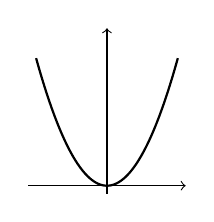
\begin{tikzpicture}[scale=0.5]
        % axis
        \draw[->] (-2,0) -- (2, 0);
        \draw[->] (0,-0.2) -- (0, 4);
        % \node[below] at (3.1,0) {$r$};
    
        \draw[domain=-1.8:1.8,thick,samples=100] plot (\x,{\x*\x});
    
    \end{tikzpicture}
    \caption{抛物势}
\end{figure}
势函数
\begin{align}
    V(x) = a x^2,
\end{align}
称为\boldtext{抛物线} parabolic 势函数。
% 【刚才是???,有什么不一样】
% 【求得波函数???】
\chat{%
刚才通过化学键的定义,引出了量子体系。换个角度,量子谐振子有什么不同?我们能从公设推知微观粒子的行为,前提是确立状态方程、求解波函数,其中状态方程中最重要的系统依赖项就是势函数。上周的一维量子体系是简单的量子状态,要么为 0,要么是有限值,所有的复杂情况都来自边界条件,由边条件可以推知所有的物理。

今天要求解的量子体系,势函数是显式地依赖于坐标的。求解之前有个问题,$a$ 表示的是什么物理量。
}
\begin{figure}[tp]\centering
    \begin{tikzpicture}[scale=0.5]
        % % axis
        % \draw[->] (-2,0) -- (2, 0);
        % \draw[->] (0,-0.2) -- (0, 4);
        % % \node[below] at (3.1,0) {$r$};
    
        \fill [pattern = north west lines] (-0.5,0) rectangle (0,2);
        \draw[thick] (0,0) -- (0,2);
        \draw[
        decoration={
            coil,
            segment length = 2mm,
            amplitude = 2mm,
            aspect = 0.5,
            post length = 1mm,
            pre length = 0.5mm},
        decorate, thick] (0,1) -- (4,1);
        \draw[fill] (4,1) circle (0.3);
    
        % \draw[domain=-1.8:1.8,thick,samples=100] plot (\x,{\x*\x});
    
        % axis
        \draw[->, fudanRed] (-1,1) -- (5, 1);
        \draw[->, fudanRed] (4,-0.5) -- (4, 2.5);
        \node[right,fudanRed] at (4,0.5) {$O$};
    
    \end{tikzpicture}
    \caption{弹簧模型}
    \end{figure}
回顾胡克定理,
% 【图,左边是墙,水平连接弹簧】,
以平衡构型建立坐标系 $O$,弹簧受到的力为 $F = -kx$,$k$ 是弹簧的劲度系数 stiffness coefficient。由牛顿力学定律
\begin{align}
    F = ma = m \pdv[2]{x}{t} = -k x
\end{align}
得到偏微分方程
\begin{align}
    \pdv[2]{x}{t} = - \frac km x,
\end{align}
很容易得到运动轨迹
\begin{align}
    x(t) = A \sin(\omega t + \delta),
\end{align}
其中 $\omega = \sqrt{\frac{k}m}$ 是振子的角频率,是体系内禀的量,$A,\delta$ 是振幅和相位,与初态有关。另外我们知道,
\begin{align}
    F(x) = -\frac{\partial V(x)}{\partial x}, 
\end{align}
解出来势能
\begin{align}
    V(x) = \int -F(x)\,\dd x = \int kx \, \dd x = \frac12 k x^2 + V_0,
\end{align}
令参考势能 $V_0 = 0$,那么势能
\begin{eqnarray}
    V(x) = \frac 12 kx^2 = \frac 12 m\omega^2 x^2.
\end{eqnarray}
由此,得到了 $a$ 的物理含义。

量子谐振子的哈密顿量,
\begin{align}
    \hat H(x) = -\frac{\hbar^2}{2m} \pdv[2]{x} + \frac 12 m\omega^2 x^2,
\end{align}
定态薛定谔方程就可以写为
\begin{align}
    -\frac{\hbar^2}{2m} \pdv[2]{\psi}{x} + \frac 12 m\omega^2 x^2 = E\psi,
    \label{eq:harm_seq_original}
\end{align}
看起来有点太复杂了,能否简化其中的常数?

\section{方程简化}

两边同除以 $-\frac{\hbar^2}{2m}$,
\begin{align}
    \pdv[2]{\psi}{x} - \frac{m^2\omega^2 x^2}{\hbar^2} \psi = \frac{-2mE}{\hbar^2}\psi,
\end{align}
归并到左边,有
\begin{align}
    \pdv[2]{\psi(x)}{x} + \left(
        \frac{2mE}{\hbar^2} - \frac{m^2\omega^2}{\hbar^2} x^2
    \right) \psi = 0,
\end{align}
设 $a = \frac{m\omega}{\hbar}$,有
\begin{align}
    \pdv[2]{\psi(x)}{x} + \left(
        \frac{2mE}{\hbar^2} - a^2 x^2
    \right) \psi = 0,
    \label{eq:harm_seq_a}
\end{align}
利用函数变量代换的规则,定义新的变量 $y = kx$,即 $x = \frac 1k y$,那么波函数 $\psi(x) = \psi(y)$,利用链式法则
\begin{align}
    &\pdv{\psi(x)}{x} = \pdv{\psi(y)}{y} \pdv yx = k \pdv{\psi(y)} {y},
    &\pdv[2]{\psi(x)}{x} = k^2 \pdv[2]{\psi(y)}{y},
\end{align}
代回薛定谔方程 \eqref{eq:harm_seq_a}
\begin{align}
    k^2 \pdv[2]{\psi(y)}{y} + \left(
        \frac{2mE}{\hbar^2} - \frac{a^2}{k^2} y^2
    \right) \psi(y) &= 0 \\
    \pdv[2]{\psi(y)}{y} + \left(
        \frac{2mE}{\hbar^2} - \frac{a^2}{k^4} y^2
    \right) \psi(y) &= 0
\end{align}
之前对 $k$ 是没有要求的,这里为了化简系数,令 $y^2$ 项前的系数为 1,设 $k^4 = a^2$,有 $y = \sqrt a x$,得到
\begin{align}
    \pdv[2]{\psi(y)}{y} + \left(
        \frac{2mE}{\hbar^2} - y^2
    \right) \psi(y) &= 0
\end{align}
其中还有一项
\begin{eqnarray}
    \frac{2mE}{a\hbar^2} = \frac{2mE}{m\omega\hbar^2} = \frac{2E}{\hbar\omega} = \lambda,
\end{eqnarray}
有
\begin{align}
    \pdv[2]{\psi(y)}{y} + (\lambda - y^2) \psi(y) = 0,
    \label{eq:harm_seq_lambda_y}
\end{align}
% 【标记了原始 Seq (1),上式为 2】
这种偏微分方程叫做变系数二阶常微分方程,这就是谐振子的\boldtext{标准方程}。

\chat{%
这个方程有很多种解法,已经被研究得很透彻了,这里讲一个标准做法。

为了求解,有必要对这个微分方程的轮廓有认知。
首先遇到的问题,是否有对称性,或者说具有什么样的对称性?
}
% 第二节
% 【】
\section{波函数的对称性}
由势函数可知
\begin{align}
    V(x) = V(-x),
\end{align}
因此对应的本征波函数 $\psi(x)$ 即 $\psi(y)$ 有确定的宇称,那么波函数要么是奇函数 $\psi(x) = -\psi(-x)$、要么是偶函数 $\psi(x) = \psi(-x)$。
\homework{\textbf{4.1} ~ (a) 对于一维的宇称算符
\begin{align}
    \hat\Pi \psi(x) = \psi(x),
\end{align}
证明 $\hat \Pi$ 是 Hermit 算符,

(b) 证明,当 $V(x) = V(-x)$ 时,$[\hat H, \hat \Pi] = 0$,

(c) 考察 $[\hat T, \hat V]$ 是否为 0,并进一步考察 $[\hat T, \hat H]$、$[\hat V, \hat H]$ 是否为 0。
}

\section{无穷远处的渐进性质}
为了求解方程,先尝试求极限情况。

当 $x \rightarrow \pm \infty$,即 $y \rightarrow \pm \infty$,$y^2 \gg \lambda$,有
\begin{align}
    \frac{\partial^2 \varphi(y)}{\partial y^2}+\left(\lambda-y^2\right) \varphi(y)=0 \Rightarrow \frac{\partial^2 \varphi(y)}{\partial y^2}-y^2 \varphi(y)=0,
\end{align}

设 $\psi(y) = \ee^{sy}$,它非奇非偶,不满足。换一种波函数,设 $\psi(y) = \ee^{sy^2}$,如果要满足品优波函数的性质,$s<0$,所以直接设为 $\psi(y) = \ee^{-sy^2} (s>0)$,求导有
\begin{align}
    &\frac{\partial}{\partial y} \ee^{-sy^2} = -2sy \, \ee^{-sy^2}, \\
    &\pdv[2]{\psi(y)}{y} = -2 s\, \ee^{-s y^2} + 4 s^2 y^2 \ee^{-s y^2},
\end{align}
\begin{lstlisting}
    D[Exp[-s y^2], y]
    D[Exp[-s y^2], {y, 2}]
    >> -2 E^(-s y^2) s y
    >> -2 E^(-s y^2) s + 4 E^(-s y^2) s^2 y^2
    \end{lstlisting}
代回原式有
\begin{align}
    4s^2 y^2 \, \ee^{-sy^2} - y^2 \ee^{-sy^2} - 2 s \ee^{-sy^2} &= 0 \\
    4s^2 y^2 \, \ee^{-sy^2} - y^2 \ee^{-sy^2} &= 0, \\
    4 s^2 & = 1,
\end{align}
解得 $s = \frac12$。得到了波函数在无穷远处的渐进性为,
\begin{equation}
    \psi(y) |_{y \rightarrow \pm\infty} = \ee^{-y^2/2}.
\end{equation}
\section{引入 Hermite 方程}
波函数可以写为
\begin{equation}
    \psi(y) = f(y) \ee^{-y^2/2},
\end{equation}
问题转化成了求解 $f(y)$。

当$y\rightarrow\pm\infty$ 时,$f(y) \rightarrow A$ 常数,才能确保 $\psi$ 的渐进行为。重新求导 
% % []
% \begin{align}
%     \pdv[2]{\psi(y)}{y} + (\lambda - y^2) \psi(y) = 0, 
% \end{align}
% []
% \begin{align}
%     \psi(y) = f(y) \, \ee^{-y^2/2},
% \end{align}
% $f(y)$ 为待求解函数,当 $y \rightarrow \pm\infty$ 时,$f(y) = A$,$\psi(y) \rightarrow \ee^{-y^2/2}$,
% 偏导为
\begin{align}
    &\frac{\partial \varphi(y)}{\partial y}=\frac{\partial f(y) e^{-y^2/2}}{\partial y}=f(y) e^{-y^2 / 2}-y e^{-y^2 / 2} f(y) \\
    &\frac{\partial^2 \varphi(y)}{\partial y^2}=f^{\prime \prime}(y) e^{-y^2 / 2}-2 y e^{-y^2 / 2} f^{\prime}(y)+\left(y^2-1\right) e^{-y^2 / 2} f(y)
\end{align}
\begin{lstlisting}
Clear[f, y]
D[f[y] Exp[-y^2/2], y] // Simplify
D[f[y] Exp[-y^2/2], {y, 2}] // Simplify
>> E^(-(y^2/2)) (-y f[y] + Derivative[1][f][y])
>> E^(-(y^2/2)) 
    ((-1 + y^2) f[y] - 2 y Derivative[1][f][y] 
    + (f^\[Prime]\[Prime])[y])
\end{lstlisting}
代回到 \eqref{eq:harm_seq_lambda_y} 中,
\begin{align}
    f^{\prime \prime}(y) e^{-y^2 / 2}-2 y e^{-y^2 / 2} f^{\prime}(y)+(\lambda-1) e^{-y^2 / 2} f(y)=0
\end{align}
% [][]Hermite 方程。
% 【】【】【4式】
稍微化简即可得另一个变系数常微分方程,
\begin{align}
    f''(y) - 2y f'(y) + (\lambda - 1) f(y) = 0, 
    \label{eq:harm_lambda_y_simp} %eq4 in course
\end{align}
称其为 Hermite 方程。

\chat{%
回到初始薛定谔方程,引入变量代换可以得到变系数常微分方程。很自然的问题是,
为什么我们要做如此多步的方程演化?换句话说,我们可否直接求 \eqref{eq:harm_seq_original} 或 \eqref{eq:harm_seq_lambda_y}?为什么变换之后求解更方便?

物化里面可能讲过,下面将会用到幂级数展开法。
}

\section{幂级数展开法}
将函数作级数展开,
\begin{align}
    &f(y) = \sum_{n=0}^\infty c_n y^n = c_0 + c_1 y + c_2 y^2 + \cdots,\\
    &f'(y) = \sum_{n=1}^\infty n c_n y^{n-1}, \\
    &f''(y) = \sum_{n=2}^\infty n(n-1) c_n y^{n-2},
\end{align}
将幂级数代回 \eqref{eq:harm_lambda_y_simp},
% 【label 5,6】
% 代回【?】,
导数的下限取值从 1、2 开始,写成从 0 开始是完全一样的,
\begin{align}
    & \sum_{n=2}^{\infty} n(n-1) c_n y^{n-2}-2 y \sum_{n=1}^{\infty} n c_n y^{n-1}+(\lambda-1) \sum_{n=0}^{\infty} c_n y^n \\
    =& \sum_{n=2}^n n(n-1) c_n y^{n-2}-\sum_{n=1}^{\infty} 2 n c_n y^n+\sum_{n=0}^{\infty}(\lambda-1) c_n y^n \\
    =& \sum_{n=2}^n n(n-1) c_n y^{n-2}-\sum_{n=0}^{\infty}(2 n-\lambda+1) c_n y^n
\end{align}
设 $m=n-2$,有
\begin{align}
    \sum_{m=0}^{\infty}(m+2)(m+1) c_{m+2} y^m-\sum_{n=0}^{\infty}(2 n-\lambda+1) c_n y^n
\end{align}
设 $n=m$,再把变量换回 $n$,有
\begin{align}
    &\sum_{n=0}^{\infty}(n+2)(n+1) c_{n+2} y^n-\sum_{n=0}^{\infty}(2 n-\lambda+1) c_n y^n \\
    ={}&\sum_{n=0}^{\infty}\left[(n+2)(n+1) c_{n+2}-(2 n-\lambda+1) c_n\right] y^n = 0, 
\end{align}
上式为 0,意味着其中每一项都要相等,
\begin{align}
    (n+2)(n+1) c_{n+2} = (2n - \lambda + 1)c_n,
\end{align}
便得到了双间隔的递推公式
\begin{align}
    c_{n+2} = \frac{2n - \lambda + 1}{(n+2)(n+1)} c_n, \quad n = 0, 1,2, \cdots,
\end{align}

做两件事,(1) 从 $c_0$ 开始推,
\begin{align}
    &n =0, \quad c_2 = \frac{1-\lambda}{2-1} c_0, \\
    &n=2, \quad c_4 = \frac{4 + 1 - \lambda}{4\times 3} c_2 = \frac{(1-\lambda)(4+1 - \lambda)}{4\times3\times2\times1} c_0, \\
    &n = 4, \quad c_6 = \frac{(1-\lambda) (4+1-\lambda) (8+1-\lambda)}{6!} c_0,
\end{align}
\begin{lstlisting}
(* 递归求解系数 *)
    Clear[c];
c[n_] := (2 (n - 2) - \[Lambda] + 1)/(n (n - 1)) c[n - 2]
c[0] := c0;
Table[c[2 i], {i, 1, 5}]
>> {1/2 c0 (1 - \[Lambda]), 
    1/24 c0 (1 - \[Lambda]) (5 - \[Lambda]), 
    1/720 c0 (1 - \[Lambda]) (5 - \[Lambda]) (9 - \[Lambda]), (
    c0 (1 - \[Lambda]) (5 - \[Lambda]) (9 - \[Lambda]) (13 - \
\[Lambda]))/40320, (1/3628800)
    c0 (1 - \[Lambda]) (5 - \[Lambda]) (9 - \[Lambda]) (13 - \[Lambda]) \
(17 - \[Lambda])}
\end{lstlisting}
% 于是
相当于给出
\begin{multline}
    f_0(y) = 
    \left[
        1 + \frac{1-\lambda}{2!} y^2 + 
        \frac{(1-\lambda) (4+1 - \lambda)}{4!} y^4 \right. \\
        \left.+ \frac{(1-\lambda) (4+1-\lambda) (8+1-\lambda)}{6!} y^6 + \cdots
    \right] c_0,
\end{multline}

(2) 从 $c_1$ 开始递推,不再具体讲了,最后结果是
\begin{multline}
    f_1(y) = \left[y + \frac{2+1 - \lambda} {3!} y^3 + \frac{(2+1-\lambda)(6+1 -\lambda)}{5!} y^5 \right. \\
    \left.+ \frac{(2+1-\lambda)(6+1-\lambda)(10+1-\lambda)}{7!} y^7
    + \cdots \right] c_1,
\end{multline}

我们利用幂级数展开,求解得到了奇数和偶数情况。那么合并到一起,
\begin{align}
    f(y) = c_0 f_0(y) + c_1 f_1(y),
\end{align}
于是 Hermite 方程 \eqref{eq:harm_lambda_y_simp} 的通解为上式子。
% 【4 是 f prime prime (y) - 2 ...】
\chat{%
前面讲过,势能是偶函数,那么波函数也必然有某种确定的宇称,
要么是偶函数 $f_0$,要么是奇函数 $f_1$,不可能是线性组合,二者单独都具有宇称,一旦组合起来就破坏的宇称。
}

% 下午的课

% 上午做了些方程的简化、讨论了渐进行为、做了幂级数的展开,得到双间隔的递推公式。
% 宇称,是名词,为何作形容词?% 2022-10-10 13:34:55  Wenbin Fan @FDU
\courseTime{3 of 4, Oct 10}
考察系数在无穷大时的行为,上下同除 $n^2$,将衰减较快二次项扔掉,即
\begin{align}
    \frac{c_{n+1}}{c_n} = \frac{2n - \lambda + 1} { (n+2) (n+1)} = \frac{ \frac{2}{n} + \frac{-\lambda+1}{n^2} } { \left(1+\frac 2n\right) \left(1+\frac1n\right) } \rightarrow \frac 2n,
\end{align}
注意到指数函数的幂级数展开,
\begin{align}
    \exp y^2 = 1 + \frac{y^2}{1!} + \frac{y^4}{2!} + \cdots + \frac{y^n}{\left(\frac n2\right)!} + \frac{y^{n+2}}{\left(\frac n2 +1\right)!} + \cdots,
\end{align}
相邻系数的比例关系,
\begin{align}
    \frac{c_{n+2}}{c_n} = \frac{\left(\frac n2\right)!} {\left(\frac n2 + 1\right)!} = \frac1{\frac n2 +1} \rightarrow \frac 2n
\end{align}
当 $y\rightarrow\infty$ 时,$f_0(y)$、$f_1(y)$ 与 $\exp y^2$ 的性质主要取决于 $n$ 较大时的高次项,即当 $n$ 很大时,$\exp y^2$ 与 $f(y)$ 有相同的性质,所以二者在 $y\rightarrow\infty$ 时有相同的渐进性为,
\begin{align}
    \psi(y) = f(y) \ee^{-y^2/2} |_{y\rightarrow \infty} = \exp y^2 \exp \left(-\frac{y^2}2\right) = \exp \frac{y^2}2 \rightarrow \infty.
\end{align}
这个波函数必须满足的品优性质。品优波函数的有限性,限制 $f(y)$ 必须在某一项终止,使它成为多项式。具体来说,品优波函数的限制对 Hermite 方程
\eqref{eq:harm_lambda_y_simp}
% $f''(y) - 2 y f'(y) + (\lambda -1) f(y) = 0$
中的任意实数 $\lambda$ 提出了量子化的条件。

如果波函数有限,必须在某一项停止。只要分子上 $2n - \lambda +1$ 任何一项为 0,后面的项也全部为 0。由此解出
\begin{align}
    \lambda = 2n +1, \quad n = 0, 1, 2, 3, \cdots
\end{align}
代入 $\lambda$ 的设定,得到
\begin{align}
    \frac{2E}{\hbar\omega} = 2n+1  \ \Rightarrow \ E = \left(n+\frac12\right)\hbar\omega,
\end{align}
特别地,当 $n=0$ 时,
\begin{align}
    E_0 = \frac12\hbar \omega,
\end{align}

求解中最重要的简化步骤,是对方程 \eqref{eq:harm_seq_lambda_y} 的渐进行为思考。那么回答之前的问题,为什么要做如此多步的推导?这是个开放式的问题。

\homework{
    \textbf{4.2} ~  对于谐振子标准方程 \eqref{eq:harm_seq_lambda_y},做幂级数展开,给出系数的递推公式,并讨论能否从中得到量子化条件。

    \textbf{4.3} ~  针对谐振子 Hermite 方程 \eqref{eq:harm_lambda_y_simp},引入复变量 $\rho = y^2$,将 Hermite 方程演化为 Kummer's 微分方程,并对它做幂级数展开、给出系数的递推公式和量子化条件。
}

已经求出了量子化条件,那么此时的量子谐振子模型有什么特殊或不一样的意义、物理行为?下面做更多有趣的分析。

\section{量子化条件的分析}

量子化条件决定了量子特征,下面分析零点能。

% \subsection{零点能}

当 $n=0$ 时,只有 $c_0$ 这一项,波函数是高斯展宽。

氢分子势能面上解离的问题,再用谐振子模型重新算一次。
$\mathrm H_2$ 的劲度系数 $k = \SI{1.3E3}{\newton\per\metre}$,得到 $\omega = \sqrt{\frac km} = \SI{8.2E14}{\hertz}$,则
\begin{eqnarray}
    E_0 = \frac 12 \hbar \omega = \SI{0.27}{\electronvolt}, 
\end{eqnarray}
这与实验值是非常相符的。换句话说,对于键能比较强的键,谐振子能给出比较准确的零点能,现在广泛采用的也是谐振子模型。

\section{本征函数}
已经得到
\begin{align}
    \psi(y) = A f(y) \ee^{-y^2/2},
\end{align}
其中 $A$ 是归一化系数,也得到了 $f_0$、$f_1$ 和量子化条件,那么可以等价地给出
\begin{align}
    &\phi_0^n (y) = A f_0^n (y) \ee^{-y^2/2}, \quad\text{偶函数}\\
    &\phi_1^n (y) = A f_1^n (y) \ee^{-y^2/2}, \quad\text{奇函数}
\end{align}
现在波函数还是非常复杂的。

为了简化多项式,取 $c_n = 2^n$,利用递推公式
\begin{align}
    c_{k+2} = \frac{2k - 2n}{(k+2)(k+1)}c_k. 
\end{align}
本来是利用 $c_0$ 从小到大推进,所以很容易得到量子化条件等,但弊端是难以写出通式。现在我们反着来做,假设截断后的最高一项是 $2^n$,再从大到小推导其它系数,推导得到
\begin{align}
    H_n(y) = \sum_{m=0}^M \frac{(-1)^m n!}{m! (n-2m)!} (2y)^{n-2m}, 
\end{align}
其中 $m$ 为求和指标,$M$ 是最大值,
\begin{align}
    M = \begin{cases}
        \frac n2, \quad n = 0, 2, 4, \cdots, \\
        \frac{n-1}2, \quad n=1,3,5,\cdots,
    \end{cases}
\end{align}
那么通过反推,可以使我们的解变成很简单的形式。
该式称为 $n$ 阶 \boldtext{Hermite 多项式},
\begin{align}
    H_n(y) = (-1)^n H_n(y), \label{eq:nth_hermitian_poly}
\end{align}
写出前 $n$ 阶 Hermite 多项式,
\begin{align}
    &H_0 (y) = 1, \\
    &H_1(y) = 2y,\\
    &H_2(y) = 4 y^2 - 2, \\
    &H_3(y) = 8 y^2 - 12 y, \\
    &H_4(y) = 16 y^4 - 48 y^2 + 12, 
\end{align}
\begin{lstlisting}
(* 厄米多项式 *)
Table[HermiteH[i, y], {i, 0, 5}]
>> {1, 2 y, -2 + 4 y^2, -12 y + 8 y^3, 12 - 48 y^2 + 16 y^4, 
120 y - 160 y^3 + 32 y^5}
\end{lstlisting}
我们约束了 Hermite 多项式是有限的,并且给定了最大的值。

这种从大到小的推导,可以与从小到大的推导做一一对应,
\begin{alignat}{2}
    &f_0^0(y) = 1 &&=H_0(y),\\
    &f_0^2(y) = 1 - 2y^2  && = - \frac12 H_2(y), \\
    &f_0^4(y) = 1- 4 y^2 + \frac43 y^4 && = 12 H_4(y),
\end{alignat}
二者相差倍数关系,这个倍数可以包括在归一化系数中,所以二者是完全等价的。

% 2022-10-10 14:15:02  Wenbin Fan @FDU
% ---
我们已经通过 $M$ 包括了奇数和偶数两种情况,波函数
\begin{align}
    &\psi(y) = A f(x) \ee^{-y^2/2}, \\
    &\psi_n(y) = A_n H_n (y) \ee^{-y^2/2}, \quad n=0,1,2,\cdots, \\
    & y = ax = \sqrt{\frac{m\omega}{\hbar}} x, \quad a^2 = \frac{m\omega}\hbar,
\end{align}
\homework{\textbf{4.5} ~  
请证明
\begin{align}
    A_n = \left(\frac{m\omega}{\pi\hbar}\right)^{1/4} \frac1 {\sqrt{2^n n!}},
\end{align}
提示,可利用 Hermite 多项式生成函数
\begin{align}
    S(x,r) = \ee^{2xr -r^2} = \sum_{n=0}^{\infty} H_n(x) \frac{r^n}{n!}, 
\end{align}
来讨论,这里可参考顾樵《量子力学》P208---211。
% 电子图书见 elearning。

体系的基态\begin{align}
    \psi_0(x) &= \left(\frac{m\omega}{\pi\hbar}\right)^{1/4} \exp \left(- \frac12 \frac{m\omega}{\hbar} x^2\right)\\
    &=\left(\frac a{\sqrt{\pi}}\right)^{1/2} \exp\left(-\frac12 a^2 x^2\right),\\
    \psi_1(x) &= a \left(\frac{2a}{\sqrt{\pi}}\right)^{1/2} x \exp \left(-\frac12 a^2 x^2\right),
\end{align}
}
% 把顾的书放上去

% 2022-10-10 14:29:36  Wenbin Fan @FDU
% 休息回来
由此知道了基态形式。画出图来,基态是个高斯函数,偶函数,更高阶的情况也可以依次画出。$n=1$ 有节点,$n=2$ 有 2 个节点,那么 $n$ 有 $n$ 个节点。
\begin{lstlisting}
(* 波函数可视化 *)
m = 1; \[Omega] = 1; \[HBar] = 1;
\[Psi][n_, x_] := ((m \[Omega])/(\[Pi] \[HBar]))^(1/4) 1/Sqrt[2^n n!]
HermiteH[n, x] Exp[-1/2 (m \[Omega])/\[HBar] x^2];
Plot[Table[\[Psi][i, x], {i, 0, 3}] // Evaluate, {x, -5, 5}]
\end{lstlisting}
\homework{
    \textbf{4.6} ~  证明谐振子 $n=0,1$ 两种情况下,不确定原理成立,计算 $(\Delta x)_n^2 (\Delta p)_n^2$ 在 $n=0,1$ 的值。

    提示,
    \begin{align}
        &(\Delta x)_n^2 = \langle \psi_n | \hat x^2 | \psi_n \rangle - \langle \psi_n | \hat x | \psi_n \rangle^2, \\
        &(\Delta p)_n^2 = \langle \psi_n | \hat p^2 | \psi_n \rangle - \langle \psi_n | \hat p | \psi_n \rangle^2,
    \end{align}
}

\section{概率密度}

问题1,经典的谐振子在什么位置出现的概率最大?

这里不方便画图,直接给大家结果,密度分布为
\begin{align}
    &\rho(x) = \frac1{\pi\sqrt{A^2 - x^2}}, \\
    &\rho(0) = \frac 1{\pi A}, \quad \rho(\pm A) = +\infty
\end{align}
% 实际上推导需要用到关系式,用到胡克定律坐标和时间的关系,又知道
% \begin{align}
%     \rho(x) \dd x = \dd t / \frac{\tau}2,
% \end{align}
因为两端速度为 0,那么概率最大,最低点速度最大,概率相对小一些。
\begin{figure}[tp]\centering
    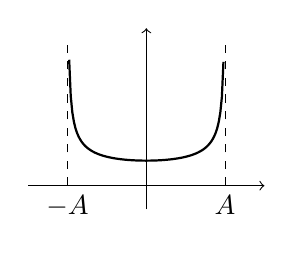
\begin{tikzpicture}[scale=1.0]
        % axis
        \draw[->] (-1.5,0) -- (1.5, 0);
        \draw[->] (0,-0.3) -- (0, 2);
    
        % % \node[below] at (3.1,0) {$r$};
    
        \draw[domain=-0.98:0.98
        ,thick,samples=100] plot (\x,{1/(pi*sqrt(1-\x*\x))});
    
        \draw[dashed] (-1, 0) -- (-1, 1.8);
        \draw[dashed] (1, 0) -- (1, 1.8);
        \node[below] at (-1,0) {$-A$};
        \node[below] at (1,0) {$A$};
    
    \end{tikzpicture}
    \caption{经典谐振子的概率密度}
\end{figure}
\suppInfo{经典谐振子的概率密度}{
从牛顿方程可以解得谐振子的轨迹
\begin{equation}
    x = A \sin (\omega t + \varphi),
\end{equation}
坐标方向的概率相当于 $\rho(x) = \frac{\dd t}{\dd x}$,反解出
\begin{equation}
    t = \frac{-\arcsin\frac{x}{A}-\varphi
   +\pi }{\omega }
\end{equation}
求导得到
\begin{eqnarray}
    \frac{\dd t}{\dd x} = -\frac{1}{\omega  \sqrt{A^2-x^2}},
\end{eqnarray}
归一化后即可得到密度分布。
}

\subsection{量子谐振子的概率密度}

经典图像中,在超出 $|A|$ 的区域中,概率是为 0 的,所以有了经典振幅的概念。

量子谐振子的波函数为
\begin{align}
    \psi_n(y) = A_n H_n(y) \exp^{-y^2/2}, \quad n=0,1,2,\cdots,
\end{align}
概率密度为模方,
\begin{align}
    |\psi_n(y)|^2 = |A_n|^2 \ee^{-y^2} |H_n (y)|^2 
    = \frac{a}{2^n n! \sqrt{\pi}} \ee^{-y^2} |H_n(y)|^2,
\end{align}

引入经典禁区 (classical restricted area) 的概念,谐振子的势能是 $V(x) = \frac 12 m\omega^2 x^2$,量子化的条件
\begin{align}
    \hbar\omega \left(n+\frac12\right) = \frac12 m\omega^2 \bar A_n^2,
\end{align}
其中 $\bar A_n$ 为量子振幅,那么
\begin{align}
    \bar A_n = \sqrt{\frac{2\hbar}{m\omega} \left(n+\frac12\right)} = \frac1a \sqrt{2n+1},
\end{align}
利用 $y=ax$,那么
\begin{align}
    \bar a_n = a \bar A_n = \sqrt{2n+1}
\end{align}
为无量纲振幅。

对于基态,
\begin{align}
    |\psi_0(y)|^2 = \frac{a}{\sqrt{\pi}} \ee^{-y^2},
\end{align}
依然是个高斯展宽,经典禁区的概率
\begin{align}
    Q_0 &= \int_{-\infty}^{-\bar A_n} |\psi_0(x)|^2 \dd x + \int_{\bar A_n}^{\infty} |\psi_0(x)|^2 \dd x \\
    &= 2 \int_{-\infty}^{-\bar A_n} |\psi_0(x)|^2 \dd x \\
    &= \frac{2}{\sqrt{\pi}} \int_{\bar a_0}^{\infty} \ee^{-y^2}\,\dd y \\
    &= \mathrm{erfc}(y),
\end{align}
% II $ x=\bar a_0 = 1$, 
同理计算出 $Q_0 = 0.157$, $Q_1 = 0.112$, $Q_2 = 0.095$, $\cdots$, $Q_{10} = 0.060$, $\cdots$。
\begin{lstlisting}
Clear["Global`*"]
\[Psi][n_, x_] := ((m \[Omega])/(\[Pi] \[HBar]))^(1/4) 1/Sqrt[2^n n!]
    HermiteH[n, 
    Sqrt[(m \[Omega])/\[HBar]] x] Exp[-1/2 (m \[Omega])/\[HBar] x^2];
n = 10;
Integrate[
    2 \[Psi][n, 
    x]^2, {x, -Infinity, -Sqrt[(2 \[HBar])/(m \[Omega]) (n + 1/2)]}, 
    Assumptions -> {m > 0, \[Omega] > 0, \[HBar] > 0}]
N[%]
>> (19634522823 Sqrt[21/\[Pi]])/(640 E^21) + Erfc[Sqrt[21]]
>> 0.0601438
\end{lstlisting}

当 $n$ 较大时,与量子情况较为接近。
\begin{lstlisting}
(* 画图,n 较大时的密度分布 *)
m = 1; \[Omega] = 1; \[HBar] = 1;
\[Psi][n_, x_] := ((m \[Omega])/(\[Pi] \[HBar]))^(1/4) 1/Sqrt[2^n n!]
    HermiteH[n, Sqrt[(m \[Omega])/\[HBar]] x] 
    Exp[-1/2 (m \[Omega])/\[HBar] x^2];
n = 10;
Plot[
    {\[Psi][n, x]^2, 
    (Pi Sqrt[(2 \[HBar])/(m \[Omega]) (n + 1/2) - x^2])^-1}, 
    {x, -6, 6}]
\end{lstlisting}

